\documentclass[12pt]{article}

\usepackage{graphicx}			% Use this package to include images
\usepackage{amsmath}			% A library of many standard math expressions
\usepackage[margin=1in]{geometry}% Sets 1in margins. 
\usepackage{fancyhdr}			% Creates headers and footers
\usepackage{enumerate}          %These two package give custom labels to a list
\usepackage[shortlabels]{enumitem}
\usepackage{matlab-prettifier}
\usepackage{tikz}
\usepackage[utf8]{inputenc}
\usepackage{pgfplots} 
\usepackage{pgfgantt}
\usepackage{pdflscape}
\usepackage{array,multirow}
\usepackage{tabularx,booktabs}
\usepackage{caption}
\newcolumntype{Y}{>{\centering\arraybackslash}X}
\usetikzlibrary{shapes.geometric}
\usetikzlibrary{arrows.meta,arrows}
\pgfplotsset{compat=newest} 
\pgfplotsset{plot coordinates/math parser=false}
\newlength\fwidth
\newlength\fheight
\usepackage{float,graphicx}
\usepackage{tikz}
\usetikzlibrary{calc,intersections}
\tikzset{ray/.style={red,-latex},object/.style={thick,blue,-latex}}
\pagestyle{fancy}
\fancyhead[l]{}
\fancyhead[c]{Experiment 3}
\fancyhead[r]{}
\fancyfoot[c]{\thepage}
\setlength{\headheight}{20pt}
\begin{document}
\author{}
\date{}
\title{Photo Electric Effect}
\maketitle
\captionsetup[figure]{labelformat=empty}
\captionsetup{justification = centering}

\section*{Aim}
To Determine Plank's constant by Photo Electric Effect and verify the the inverse square law.

\section*{Theory}
Metals when hit with radiation of certain frequencies emit electrons
\[hf = \underbrace{\frac{1}{2}mv^2}_\text{K.E of e}+e\phi \]
Substituting : $\displaystyle \frac{1}{2}mv^2= eV_s$ , we get

\[V_s=\frac{h}{e}f - \phi\]

\section*{Analysis}
In theory, the value for stopping potential should not differ for any value of intensity or distance.
First we look at the data of stopping voltage for high and low intensities keeping distance constant for both values.
Notice that the values are only $0.01V$ which is just the least count error.
The values only diverge for low intensity, large distance and blue filter.
Also the last value was not recorded because the current never hit zero.
This might happen because the intensity of light passing through the filter is not enough to activate the sensor.

Other than this outlier, all other values for stopping potential for high and low intensities are the same.
%Thus, we can conclude that the stopping potential does not depend on the intensity of light shined as long as it is above a certain treshold.
However we see a small difference when we vary distance.
We shall calculate the errors as the difference in readings of the two most extreme values of stopping voltage
\begin{align*}
    \text{Red : }0.25-0.24 = 0.01 \\
    \text{Yellow 1 : }0.45-0.43 = 0.02 \\
    \text{Yellow 2 : }0.51-0.49 = 0.02 \\
    \text{Green : }0.62-0.55 = 0.07 \\ 
    \text{Blue : }0.74-0.65 = 0.09 \\
\end{align*}

\begin{figure}[!ht]
    \centering
    \caption{Fitting for both cases}
    \setlength\fwidth{0.6\textwidth}
    \setlength\fheight{0.5\textwidth}
    % This file was created by matlab2tikz.
%
\definecolor{mycolor1}{rgb}{0.85000,0.32500,0.09800}%
\definecolor{mycolor2}{rgb}{0.12941,0.12941,0.12941}%
%
\begin{tikzpicture}

\begin{axis}[%
width=0.951\fwidth,
height=\fheight,
at={(0\fwidth,0\fheight)},
scale only axis,
xmin=300000000000000,
xmax=700000000000000,
xlabel style={font=\color{mycolor2}},
xlabel={Frequency (for 25 cm)},
ymin=-0.4,
ymax=1,
ylabel style={font=\color{mycolor2}},
ylabel={Stopping Potential},
axis background/.style={fill=white},
xmajorgrids,
ymajorgrids,
legend style={at={(0.03,0.97)}, anchor=north west, legend cell align=left, align=left}
]
\addplot [color=blue, only marks, mark=o, mark options={solid, blue}]
 plot [error bars/.cd, y dir=both, y explicit, error bar style={line width=0.5pt}, error mark options={line width=0.5pt, mark size=6.0pt, rotate=90}]
 table[row sep=crcr, y error plus index=2, y error minus index=3]{%
472114107086614	0.25	0.01	0.01\\
525951680701754	0.44	0.02	0.02\\
555171218518518	0.5	0.02	0.02\\
599584916000000	0.58	0.07	0.07\\
651722734782609	0.73	0.09	0.09\\
};
\addlegendentry{Data}

\addplot [color=mycolor1]
  table[row sep=crcr]{%
300000000000000	-0.262090286872451\\
301000000000000	-0.259093536729472\\
302000000000000	-0.256096786586493\\
303000000000000	-0.253100036443514\\
304000000000000	-0.250103286300535\\
305000000000000	-0.247106536157555\\
306000000000000	-0.244109786014576\\
307000000000000	-0.241113035871597\\
308000000000000	-0.238116285728618\\
309000000000000	-0.235119535585639\\
310000000000000	-0.23212278544266\\
311000000000000	-0.229126035299681\\
312000000000000	-0.226129285156701\\
313000000000000	-0.223132535013722\\
314000000000000	-0.220135784870743\\
315000000000000	-0.217139034727764\\
316000000000000	-0.214142284584785\\
317000000000000	-0.211145534441806\\
318000000000000	-0.208148784298827\\
319000000000000	-0.205152034155848\\
320000000000000	-0.202155284012869\\
321000000000000	-0.199158533869889\\
322000000000000	-0.19616178372691\\
323000000000000	-0.193165033583931\\
324000000000000	-0.190168283440952\\
325000000000000	-0.187171533297973\\
326000000000000	-0.184174783154994\\
327000000000000	-0.181178033012015\\
328000000000000	-0.178181282869036\\
329000000000000	-0.175184532726056\\
330000000000000	-0.172187782583077\\
331000000000000	-0.169191032440098\\
332000000000000	-0.166194282297119\\
333000000000000	-0.16319753215414\\
334000000000000	-0.160200782011161\\
335000000000000	-0.157204031868182\\
336000000000000	-0.154207281725202\\
337000000000000	-0.151210531582223\\
338000000000000	-0.148213781439244\\
339000000000000	-0.145217031296265\\
340000000000000	-0.142220281153286\\
341000000000000	-0.139223531010307\\
342000000000000	-0.136226780867328\\
343000000000000	-0.133230030724349\\
344000000000000	-0.13023328058137\\
345000000000000	-0.12723653043839\\
346000000000000	-0.124239780295411\\
347000000000000	-0.121243030152432\\
348000000000000	-0.118246280009453\\
349000000000000	-0.115249529866474\\
350000000000000	-0.112252779723495\\
351000000000000	-0.109256029580516\\
352000000000000	-0.106259279437537\\
353000000000000	-0.103262529294557\\
354000000000000	-0.100265779151578\\
355000000000000	-0.0972690290085991\\
356000000000000	-0.0942722788656201\\
357000000000000	-0.0912755287226408\\
358000000000000	-0.0882787785796617\\
359000000000000	-0.0852820284366826\\
360000000000000	-0.0822852782937034\\
361000000000000	-0.0792885281507243\\
362000000000000	-0.0762917780077452\\
363000000000000	-0.0732950278647662\\
364000000000000	-0.0702982777217869\\
365000000000000	-0.0673015275788078\\
366000000000000	-0.0643047774358287\\
367000000000000	-0.0613080272928497\\
368000000000000	-0.0583112771498704\\
369000000000000	-0.0553145270068913\\
370000000000000	-0.0523177768639123\\
371000000000000	-0.049321026720933\\
372000000000000	-0.0463242765779539\\
373000000000000	-0.0433275264349748\\
374000000000000	-0.0403307762919958\\
375000000000000	-0.0373340261490165\\
376000000000000	-0.0343372760060374\\
377000000000000	-0.0313405258630584\\
378000000000000	-0.0283437757200791\\
379000000000000	-0.0253470255771\\
380000000000000	-0.0223502754341209\\
381000000000000	-0.0193535252911419\\
382000000000000	-0.0163567751481626\\
383000000000000	-0.0133600250051835\\
384000000000000	-0.0103632748622045\\
385000000000000	-0.00736652471922539\\
386000000000000	-0.0043697745762461\\
387000000000000	-0.00137302443326703\\
388000000000000	0.00162372570971203\\
389000000000000	0.00462047585269132\\
390000000000000	0.00761722599567038\\
391000000000000	0.0106139761386495\\
392000000000000	0.0136107262816285\\
393000000000000	0.0166074764246078\\
394000000000000	0.0196042265675869\\
395000000000000	0.0226009767105659\\
396000000000000	0.0255977268535452\\
397000000000000	0.0285944769965243\\
398000000000000	0.0315912271395034\\
399000000000000	0.0345879772824824\\
400000000000000	0.0375847274254617\\
401000000000000	0.0405814775684408\\
402000000000000	0.0435782277114198\\
403000000000000	0.0465749778543989\\
404000000000000	0.0495717279973782\\
405000000000000	0.0525684781403573\\
406000000000000	0.0555652282833363\\
407000000000000	0.0585619784263156\\
408000000000000	0.0615587285692947\\
409000000000000	0.0645554787122737\\
410000000000000	0.0675522288552528\\
411000000000000	0.0705489789982321\\
412000000000000	0.0735457291412112\\
413000000000000	0.0765424792841902\\
414000000000000	0.0795392294271693\\
415000000000000	0.0825359795701486\\
416000000000000	0.0855327297131276\\
417000000000000	0.0885294798561067\\
418000000000000	0.091526229999086\\
419000000000000	0.0945229801420651\\
420000000000000	0.0975197302850441\\
421000000000000	0.100516480428023\\
422000000000000	0.103513230571002\\
423000000000000	0.106509980713982\\
424000000000000	0.109506730856961\\
425000000000000	0.11250348099994\\
426000000000000	0.115500231142919\\
427000000000000	0.118496981285898\\
428000000000000	0.121493731428877\\
429000000000000	0.124490481571856\\
430000000000000	0.127487231714835\\
431000000000000	0.130483981857815\\
432000000000000	0.133480732000794\\
433000000000000	0.136477482143773\\
434000000000000	0.139474232286752\\
435000000000000	0.142470982429731\\
436000000000000	0.14546773257271\\
437000000000000	0.148464482715689\\
438000000000000	0.151461232858668\\
439000000000000	0.154457983001647\\
440000000000000	0.157454733144627\\
441000000000000	0.160451483287606\\
442000000000000	0.163448233430585\\
443000000000000	0.166444983573564\\
444000000000000	0.169441733716543\\
445000000000000	0.172438483859522\\
446000000000000	0.175435234002501\\
447000000000000	0.178431984145481\\
448000000000000	0.18142873428846\\
449000000000000	0.184425484431439\\
450000000000000	0.187422234574418\\
451000000000000	0.190418984717397\\
452000000000000	0.193415734860376\\
453000000000000	0.196412485003355\\
454000000000000	0.199409235146335\\
455000000000000	0.202405985289314\\
456000000000000	0.205402735432293\\
457000000000000	0.208399485575272\\
458000000000000	0.211396235718251\\
459000000000000	0.21439298586123\\
460000000000000	0.217389736004209\\
461000000000000	0.220386486147188\\
462000000000000	0.223383236290168\\
463000000000000	0.226379986433147\\
464000000000000	0.229376736576126\\
465000000000000	0.232373486719105\\
466000000000000	0.235370236862084\\
467000000000000	0.238366987005063\\
468000000000000	0.241363737148042\\
469000000000000	0.244360487291021\\
470000000000000	0.247357237434001\\
471000000000000	0.25035398757698\\
472000000000000	0.253350737719959\\
473000000000000	0.256347487862938\\
474000000000000	0.259344238005917\\
475000000000000	0.262340988148896\\
476000000000000	0.265337738291875\\
477000000000000	0.268334488434854\\
478000000000000	0.271331238577833\\
479000000000000	0.274327988720813\\
480000000000000	0.277324738863792\\
481000000000000	0.280321489006771\\
482000000000000	0.28331823914975\\
483000000000000	0.286314989292729\\
484000000000000	0.289311739435708\\
485000000000000	0.292308489578687\\
486000000000000	0.295305239721666\\
487000000000000	0.298301989864646\\
488000000000000	0.301298740007625\\
489000000000000	0.304295490150604\\
490000000000000	0.307292240293583\\
491000000000000	0.310288990436562\\
492000000000000	0.313285740579541\\
493000000000000	0.31628249072252\\
494000000000000	0.3192792408655\\
495000000000000	0.322275991008479\\
496000000000000	0.325272741151458\\
497000000000000	0.328269491294437\\
498000000000000	0.331266241437416\\
499000000000000	0.334262991580395\\
500000000000000	0.337259741723374\\
501000000000000	0.340256491866354\\
502000000000000	0.343253242009333\\
503000000000000	0.346249992152312\\
504000000000000	0.349246742295291\\
505000000000000	0.35224349243827\\
506000000000000	0.355240242581249\\
507000000000000	0.358236992724228\\
508000000000000	0.361233742867207\\
509000000000000	0.364230493010187\\
510000000000000	0.367227243153166\\
511000000000000	0.370223993296145\\
512000000000000	0.373220743439124\\
513000000000000	0.376217493582103\\
514000000000000	0.379214243725082\\
515000000000000	0.382210993868061\\
516000000000000	0.38520774401104\\
517000000000000	0.388204494154019\\
518000000000000	0.391201244296999\\
519000000000000	0.394197994439978\\
520000000000000	0.397194744582957\\
521000000000000	0.400191494725936\\
522000000000000	0.403188244868915\\
523000000000000	0.406184995011894\\
524000000000000	0.409181745154873\\
525000000000000	0.412178495297852\\
526000000000000	0.415175245440832\\
527000000000000	0.418171995583811\\
528000000000000	0.42116874572679\\
529000000000000	0.424165495869769\\
530000000000000	0.427162246012748\\
531000000000000	0.430158996155727\\
532000000000000	0.433155746298706\\
533000000000000	0.436152496441685\\
534000000000000	0.439149246584665\\
535000000000000	0.442145996727644\\
536000000000000	0.445142746870623\\
537000000000000	0.448139497013602\\
538000000000000	0.451136247156581\\
539000000000000	0.45413299729956\\
540000000000000	0.457129747442539\\
541000000000000	0.460126497585519\\
542000000000000	0.463123247728498\\
543000000000000	0.466119997871477\\
544000000000000	0.469116748014456\\
545000000000000	0.472113498157435\\
546000000000000	0.475110248300414\\
547000000000000	0.478106998443393\\
548000000000000	0.481103748586373\\
549000000000000	0.484100498729352\\
550000000000000	0.487097248872331\\
551000000000000	0.49009399901531\\
552000000000000	0.493090749158289\\
553000000000000	0.496087499301268\\
554000000000000	0.499084249444247\\
555000000000000	0.502080999587226\\
556000000000000	0.505077749730205\\
557000000000000	0.508074499873185\\
558000000000000	0.511071250016164\\
559000000000000	0.514068000159143\\
560000000000000	0.517064750302122\\
561000000000000	0.520061500445101\\
562000000000000	0.52305825058808\\
563000000000000	0.526055000731059\\
564000000000000	0.529051750874038\\
565000000000000	0.532048501017018\\
566000000000000	0.535045251159997\\
567000000000000	0.538042001302976\\
568000000000000	0.541038751445955\\
569000000000000	0.544035501588934\\
570000000000000	0.547032251731913\\
571000000000000	0.550029001874892\\
572000000000000	0.553025752017871\\
573000000000000	0.55602250216085\\
574000000000000	0.55901925230383\\
575000000000000	0.562016002446809\\
576000000000000	0.565012752589788\\
577000000000000	0.568009502732767\\
578000000000000	0.571006252875746\\
579000000000000	0.574003003018725\\
580000000000000	0.576999753161704\\
581000000000000	0.579996503304684\\
582000000000000	0.582993253447663\\
583000000000000	0.585990003590642\\
584000000000000	0.588986753733621\\
585000000000000	0.5919835038766\\
586000000000000	0.594980254019579\\
587000000000000	0.597977004162558\\
588000000000000	0.600973754305538\\
589000000000000	0.603970504448517\\
590000000000000	0.606967254591496\\
591000000000000	0.609964004734475\\
592000000000000	0.612960754877454\\
593000000000000	0.615957505020433\\
594000000000000	0.618954255163412\\
595000000000000	0.621951005306391\\
596000000000000	0.624947755449371\\
597000000000000	0.62794450559235\\
598000000000000	0.630941255735329\\
599000000000000	0.633938005878308\\
600000000000000	0.636934756021287\\
601000000000000	0.639931506164266\\
602000000000000	0.642928256307245\\
603000000000000	0.645925006450224\\
604000000000000	0.648921756593204\\
605000000000000	0.651918506736183\\
606000000000000	0.654915256879162\\
607000000000000	0.657912007022141\\
608000000000000	0.66090875716512\\
609000000000000	0.663905507308099\\
610000000000000	0.666902257451078\\
611000000000000	0.669899007594057\\
612000000000000	0.672895757737036\\
613000000000000	0.675892507880016\\
614000000000000	0.678889258022995\\
615000000000000	0.681886008165974\\
616000000000000	0.684882758308953\\
617000000000000	0.687879508451932\\
618000000000000	0.690876258594911\\
619000000000000	0.69387300873789\\
620000000000000	0.696869758880869\\
621000000000000	0.699866509023849\\
622000000000000	0.702863259166828\\
623000000000000	0.705860009309807\\
624000000000000	0.708856759452786\\
625000000000000	0.711853509595765\\
626000000000000	0.714850259738744\\
627000000000000	0.717847009881723\\
628000000000000	0.720843760024703\\
629000000000000	0.723840510167682\\
630000000000000	0.726837260310661\\
631000000000000	0.72983401045364\\
632000000000000	0.732830760596619\\
633000000000000	0.735827510739598\\
634000000000000	0.738824260882577\\
635000000000000	0.741821011025557\\
636000000000000	0.744817761168536\\
637000000000000	0.747814511311515\\
638000000000000	0.750811261454494\\
639000000000000	0.753808011597473\\
640000000000000	0.756804761740452\\
641000000000000	0.759801511883431\\
642000000000000	0.76279826202641\\
643000000000000	0.765795012169389\\
644000000000000	0.768791762312369\\
645000000000000	0.771788512455348\\
646000000000000	0.774785262598327\\
647000000000000	0.777782012741306\\
648000000000000	0.780778762884285\\
649000000000000	0.783775513027264\\
650000000000000	0.786772263170243\\
651000000000000	0.789769013313222\\
652000000000000	0.792765763456202\\
653000000000000	0.795762513599181\\
654000000000000	0.79875926374216\\
655000000000000	0.801756013885139\\
656000000000000	0.804752764028118\\
657000000000000	0.807749514171097\\
658000000000000	0.810746264314076\\
659000000000000	0.813743014457055\\
660000000000000	0.816739764600035\\
661000000000000	0.819736514743014\\
662000000000000	0.822733264885993\\
663000000000000	0.825730015028972\\
664000000000000	0.828726765171951\\
665000000000000	0.83172351531493\\
666000000000000	0.834720265457909\\
667000000000000	0.837717015600888\\
668000000000000	0.840713765743867\\
669000000000000	0.843710515886847\\
670000000000000	0.846707266029826\\
671000000000000	0.849704016172805\\
672000000000000	0.852700766315784\\
673000000000000	0.855697516458763\\
674000000000000	0.858694266601742\\
675000000000000	0.861691016744722\\
676000000000000	0.8646877668877\\
677000000000000	0.86768451703068\\
678000000000000	0.870681267173659\\
679000000000000	0.873678017316638\\
680000000000000	0.876674767459617\\
681000000000000	0.879671517602596\\
682000000000000	0.882668267745575\\
683000000000000	0.885665017888555\\
684000000000000	0.888661768031534\\
685000000000000	0.891658518174513\\
686000000000000	0.894655268317492\\
687000000000000	0.897652018460471\\
688000000000000	0.90064876860345\\
689000000000000	0.903645518746429\\
690000000000000	0.906642268889408\\
691000000000000	0.909639019032388\\
692000000000000	0.912635769175367\\
693000000000000	0.915632519318346\\
694000000000000	0.918629269461325\\
695000000000000	0.921626019604304\\
696000000000000	0.924622769747283\\
697000000000000	0.927619519890262\\
698000000000000	0.930616270033242\\
699000000000000	0.93361302017622\\
700000000000000	0.9366097703192\\
};
\addlegendentry{Fit}

\end{axis}
\end{tikzpicture}%
    % This file was created by matlab2tikz.
%
\definecolor{mycolor1}{rgb}{0.85000,0.32500,0.09800}%
\definecolor{mycolor2}{rgb}{0.12941,0.12941,0.12941}%
%
\begin{tikzpicture}

\begin{axis}[%
width=0.951\fwidth,
height=\fheight,
at={(0\fwidth,0\fheight)},
scale only axis,
xmin=300000000000000,
xmax=700000000000000,
xlabel style={font=\color{mycolor2}},
xlabel={Frequency (for 20 cm)},
ymin=-0.4,
ymax=1,
ylabel style={font=\color{mycolor2}},
ylabel={Stopping Potential},
axis background/.style={fill=white},
xmajorgrids,
ymajorgrids,
legend style={at={(0.03,0.97)}, anchor=north west, legend cell align=left, align=left}
]
\addplot [color=blue, only marks, mark=o, mark options={solid, blue}]
 plot [error bars/.cd, y dir=both, y explicit, error bar style={line width=0.5pt}, error mark options={line width=0.5pt, mark size=6.0pt, rotate=90}]
 table[row sep=crcr, y error plus index=2, y error minus index=3]{%
472114107086614	0.24	0.01	0.01\\
525951680701754	0.43	0.02	0.02\\
555171218518518	0.49	0.02	0.02\\
599584916000000	0.55	0.07	0.07\\
651722734782609	0.65	0.09	0.09\\
};
\addlegendentry{Data}

\addplot [color=mycolor1]
  table[row sep=crcr]{%
300000000000000	-0.257107429801492\\
301000000000000	-0.254190710390713\\
302000000000000	-0.251273990979934\\
303000000000000	-0.248357271569156\\
304000000000000	-0.245440552158377\\
305000000000000	-0.242523832747598\\
306000000000000	-0.239607113336819\\
307000000000000	-0.236690393926041\\
308000000000000	-0.233773674515262\\
309000000000000	-0.230856955104483\\
310000000000000	-0.227940235693704\\
311000000000000	-0.225023516282926\\
312000000000000	-0.222106796872147\\
313000000000000	-0.219190077461368\\
314000000000000	-0.21627335805059\\
315000000000000	-0.213356638639811\\
316000000000000	-0.210439919229032\\
317000000000000	-0.207523199818253\\
318000000000000	-0.204606480407475\\
319000000000000	-0.201689760996696\\
320000000000000	-0.198773041585917\\
321000000000000	-0.195856322175138\\
322000000000000	-0.19293960276436\\
323000000000000	-0.190022883353581\\
324000000000000	-0.187106163942802\\
325000000000000	-0.184189444532024\\
326000000000000	-0.181272725121245\\
327000000000000	-0.178356005710466\\
328000000000000	-0.175439286299687\\
329000000000000	-0.172522566888909\\
330000000000000	-0.16960584747813\\
331000000000000	-0.166689128067351\\
332000000000000	-0.163772408656572\\
333000000000000	-0.160855689245794\\
334000000000000	-0.157938969835015\\
335000000000000	-0.155022250424236\\
336000000000000	-0.152105531013457\\
337000000000000	-0.149188811602679\\
338000000000000	-0.1462720921919\\
339000000000000	-0.143355372781121\\
340000000000000	-0.140438653370343\\
341000000000000	-0.137521933959564\\
342000000000000	-0.134605214548785\\
343000000000000	-0.131688495138006\\
344000000000000	-0.128771775727228\\
345000000000000	-0.125855056316449\\
346000000000000	-0.12293833690567\\
347000000000000	-0.120021617494892\\
348000000000000	-0.117104898084113\\
349000000000000	-0.114188178673334\\
350000000000000	-0.111271459262555\\
351000000000000	-0.108354739851777\\
352000000000000	-0.105438020440998\\
353000000000000	-0.102521301030219\\
354000000000000	-0.0996045816194404\\
355000000000000	-0.0966878622086618\\
356000000000000	-0.0937711427978829\\
357000000000000	-0.0908544233871043\\
358000000000000	-0.0879377039763256\\
359000000000000	-0.0850209845655467\\
360000000000000	-0.0821042651547681\\
361000000000000	-0.0791875457439895\\
362000000000000	-0.0762708263332106\\
363000000000000	-0.0733541069224319\\
364000000000000	-0.0704373875116531\\
365000000000000	-0.0675206681008744\\
366000000000000	-0.0646039486900958\\
367000000000000	-0.0616872292793169\\
368000000000000	-0.0587705098685383\\
369000000000000	-0.0558537904577596\\
370000000000000	-0.0529370710469808\\
371000000000000	-0.0500203516362021\\
372000000000000	-0.0471036322254232\\
373000000000000	-0.0441869128146446\\
374000000000000	-0.041270193403866\\
375000000000000	-0.0383534739930871\\
376000000000000	-0.0354367545823084\\
377000000000000	-0.0325200351715298\\
378000000000000	-0.0296033157607509\\
379000000000000	-0.0266865963499723\\
380000000000000	-0.0237698769391934\\
381000000000000	-0.0208531575284148\\
382000000000000	-0.0179364381176361\\
383000000000000	-0.0150197187068573\\
384000000000000	-0.0121029992960786\\
385000000000000	-0.00918627988529996\\
386000000000000	-0.0062695604745211\\
387000000000000	-0.00335284106374245\\
388000000000000	-0.000436121652963806\\
389000000000000	0.00248059775781506\\
390000000000000	0.00539731716859371\\
391000000000000	0.00831403657937257\\
392000000000000	0.0112307559901512\\
393000000000000	0.0141474754009299\\
394000000000000	0.0170641948117087\\
395000000000000	0.0199809142224874\\
396000000000000	0.022897633633266\\
397000000000000	0.0258143530440449\\
398000000000000	0.0287310724548235\\
399000000000000	0.0316477918656024\\
400000000000000	0.034564511276381\\
401000000000000	0.0374812306871597\\
402000000000000	0.0403979500979386\\
403000000000000	0.0433146695087172\\
404000000000000	0.0462313889194959\\
405000000000000	0.0491481083302747\\
406000000000000	0.0520648277410534\\
407000000000000	0.0549815471518322\\
408000000000000	0.0578982665626109\\
409000000000000	0.0608149859733895\\
410000000000000	0.0637317053841684\\
411000000000000	0.066648424794947\\
412000000000000	0.0695651442057257\\
413000000000000	0.0724818636165045\\
414000000000000	0.0753985830272832\\
415000000000000	0.0783153024380618\\
416000000000000	0.0812320218488407\\
417000000000000	0.0841487412596194\\
418000000000000	0.0870654606703982\\
419000000000000	0.0899821800811769\\
420000000000000	0.0928988994919555\\
421000000000000	0.0958156189027344\\
422000000000000	0.098732338313513\\
423000000000000	0.101649057724292\\
424000000000000	0.104565777135071\\
425000000000000	0.107482496545849\\
426000000000000	0.110399215956628\\
427000000000000	0.113315935367407\\
428000000000000	0.116232654778185\\
429000000000000	0.119149374188964\\
430000000000000	0.122066093599743\\
431000000000000	0.124982813010521\\
432000000000000	0.1278995324213\\
433000000000000	0.130816251832079\\
434000000000000	0.133732971242858\\
435000000000000	0.136649690653637\\
436000000000000	0.139566410064415\\
437000000000000	0.142483129475194\\
438000000000000	0.145399848885973\\
439000000000000	0.148316568296751\\
440000000000000	0.15123328770753\\
441000000000000	0.154150007118309\\
442000000000000	0.157066726529087\\
443000000000000	0.159983445939866\\
444000000000000	0.162900165350645\\
445000000000000	0.165816884761424\\
446000000000000	0.168733604172203\\
447000000000000	0.171650323582981\\
448000000000000	0.17456704299376\\
449000000000000	0.177483762404539\\
450000000000000	0.180400481815317\\
451000000000000	0.183317201226096\\
452000000000000	0.186233920636875\\
453000000000000	0.189150640047654\\
454000000000000	0.192067359458432\\
455000000000000	0.194984078869211\\
456000000000000	0.19790079827999\\
457000000000000	0.200817517690768\\
458000000000000	0.203734237101547\\
459000000000000	0.206650956512326\\
460000000000000	0.209567675923105\\
461000000000000	0.212484395333883\\
462000000000000	0.215401114744662\\
463000000000000	0.218317834155441\\
464000000000000	0.22123455356622\\
465000000000000	0.224151272976998\\
466000000000000	0.227067992387777\\
467000000000000	0.229984711798556\\
468000000000000	0.232901431209334\\
469000000000000	0.235818150620113\\
470000000000000	0.238734870030892\\
471000000000000	0.241651589441671\\
472000000000000	0.24456830885245\\
473000000000000	0.247485028263228\\
474000000000000	0.250401747674007\\
475000000000000	0.253318467084786\\
476000000000000	0.256235186495564\\
477000000000000	0.259151905906343\\
478000000000000	0.262068625317122\\
479000000000000	0.2649853447279\\
480000000000000	0.267902064138679\\
481000000000000	0.270818783549458\\
482000000000000	0.273735502960237\\
483000000000000	0.276652222371015\\
484000000000000	0.279568941781794\\
485000000000000	0.282485661192573\\
486000000000000	0.285402380603352\\
487000000000000	0.28831910001413\\
488000000000000	0.291235819424909\\
489000000000000	0.294152538835688\\
490000000000000	0.297069258246466\\
491000000000000	0.299985977657245\\
492000000000000	0.302902697068024\\
493000000000000	0.305819416478803\\
494000000000000	0.308736135889581\\
495000000000000	0.31165285530036\\
496000000000000	0.314569574711139\\
497000000000000	0.317486294121918\\
498000000000000	0.320403013532696\\
499000000000000	0.323319732943475\\
500000000000000	0.326236452354254\\
501000000000000	0.329153171765032\\
502000000000000	0.332069891175811\\
503000000000000	0.33498661058659\\
504000000000000	0.337903329997369\\
505000000000000	0.340820049408147\\
506000000000000	0.343736768818926\\
507000000000000	0.346653488229705\\
508000000000000	0.349570207640484\\
509000000000000	0.352486927051262\\
510000000000000	0.355403646462041\\
511000000000000	0.35832036587282\\
512000000000000	0.361237085283598\\
513000000000000	0.364153804694377\\
514000000000000	0.367070524105156\\
515000000000000	0.369987243515935\\
516000000000000	0.372903962926713\\
517000000000000	0.375820682337492\\
518000000000000	0.378737401748271\\
519000000000000	0.38165412115905\\
520000000000000	0.384570840569828\\
521000000000000	0.387487559980607\\
522000000000000	0.390404279391386\\
523000000000000	0.393320998802164\\
524000000000000	0.396237718212943\\
525000000000000	0.399154437623722\\
526000000000000	0.402071157034501\\
527000000000000	0.404987876445279\\
528000000000000	0.407904595856058\\
529000000000000	0.410821315266837\\
530000000000000	0.413738034677616\\
531000000000000	0.416654754088394\\
532000000000000	0.419571473499173\\
533000000000000	0.422488192909952\\
534000000000000	0.42540491232073\\
535000000000000	0.428321631731509\\
536000000000000	0.431238351142288\\
537000000000000	0.434155070553067\\
538000000000000	0.437071789963845\\
539000000000000	0.439988509374624\\
540000000000000	0.442905228785403\\
541000000000000	0.445821948196182\\
542000000000000	0.44873866760696\\
543000000000000	0.451655387017739\\
544000000000000	0.454572106428518\\
545000000000000	0.457488825839297\\
546000000000000	0.460405545250075\\
547000000000000	0.463322264660854\\
548000000000000	0.466238984071633\\
549000000000000	0.469155703482411\\
550000000000000	0.47207242289319\\
551000000000000	0.474989142303969\\
552000000000000	0.477905861714748\\
553000000000000	0.480822581125526\\
554000000000000	0.483739300536305\\
555000000000000	0.486656019947084\\
556000000000000	0.489572739357863\\
557000000000000	0.492489458768641\\
558000000000000	0.49540617817942\\
559000000000000	0.498322897590199\\
560000000000000	0.501239617000977\\
561000000000000	0.504156336411756\\
562000000000000	0.507073055822535\\
563000000000000	0.509989775233314\\
564000000000000	0.512906494644092\\
565000000000000	0.515823214054871\\
566000000000000	0.51873993346565\\
567000000000000	0.521656652876429\\
568000000000000	0.524573372287207\\
569000000000000	0.527490091697986\\
570000000000000	0.530406811108765\\
571000000000000	0.533323530519543\\
572000000000000	0.536240249930322\\
573000000000000	0.539156969341101\\
574000000000000	0.54207368875188\\
575000000000000	0.544990408162658\\
576000000000000	0.547907127573437\\
577000000000000	0.550823846984216\\
578000000000000	0.553740566394995\\
579000000000000	0.556657285805773\\
580000000000000	0.559574005216552\\
581000000000000	0.562490724627331\\
582000000000000	0.565407444038109\\
583000000000000	0.568324163448888\\
584000000000000	0.571240882859667\\
585000000000000	0.574157602270446\\
586000000000000	0.577074321681224\\
587000000000000	0.579991041092003\\
588000000000000	0.582907760502782\\
589000000000000	0.585824479913561\\
590000000000000	0.588741199324339\\
591000000000000	0.591657918735118\\
592000000000000	0.594574638145897\\
593000000000000	0.597491357556675\\
594000000000000	0.600408076967454\\
595000000000000	0.603324796378233\\
596000000000000	0.606241515789012\\
597000000000000	0.60915823519979\\
598000000000000	0.612074954610569\\
599000000000000	0.614991674021348\\
600000000000000	0.617908393432127\\
601000000000000	0.620825112842905\\
602000000000000	0.623741832253684\\
603000000000000	0.626658551664463\\
604000000000000	0.629575271075241\\
605000000000000	0.63249199048602\\
606000000000000	0.635408709896799\\
607000000000000	0.638325429307578\\
608000000000000	0.641242148718356\\
609000000000000	0.644158868129135\\
610000000000000	0.647075587539914\\
611000000000000	0.649992306950693\\
612000000000000	0.652909026361471\\
613000000000000	0.65582574577225\\
614000000000000	0.658742465183029\\
615000000000000	0.661659184593807\\
616000000000000	0.664575904004586\\
617000000000000	0.667492623415365\\
618000000000000	0.670409342826144\\
619000000000000	0.673326062236922\\
620000000000000	0.676242781647701\\
621000000000000	0.67915950105848\\
622000000000000	0.682076220469259\\
623000000000000	0.684992939880037\\
624000000000000	0.687909659290816\\
625000000000000	0.690826378701595\\
626000000000000	0.693743098112373\\
627000000000000	0.696659817523152\\
628000000000000	0.699576536933931\\
629000000000000	0.70249325634471\\
630000000000000	0.705409975755488\\
631000000000000	0.708326695166267\\
632000000000000	0.711243414577046\\
633000000000000	0.714160133987825\\
634000000000000	0.717076853398603\\
635000000000000	0.719993572809382\\
636000000000000	0.722910292220161\\
637000000000000	0.72582701163094\\
638000000000000	0.728743731041718\\
639000000000000	0.731660450452497\\
640000000000000	0.734577169863276\\
641000000000000	0.737493889274054\\
642000000000000	0.740410608684833\\
643000000000000	0.743327328095612\\
644000000000000	0.746244047506391\\
645000000000000	0.749160766917169\\
646000000000000	0.752077486327948\\
647000000000000	0.754994205738727\\
648000000000000	0.757910925149506\\
649000000000000	0.760827644560284\\
650000000000000	0.763744363971063\\
651000000000000	0.766661083381842\\
652000000000000	0.76957780279262\\
653000000000000	0.772494522203399\\
654000000000000	0.775411241614178\\
655000000000000	0.778327961024956\\
656000000000000	0.781244680435735\\
657000000000000	0.784161399846514\\
658000000000000	0.787078119257293\\
659000000000000	0.789994838668072\\
660000000000000	0.79291155807885\\
661000000000000	0.795828277489629\\
662000000000000	0.798744996900408\\
663000000000000	0.801661716311186\\
664000000000000	0.804578435721965\\
665000000000000	0.807495155132744\\
666000000000000	0.810411874543522\\
667000000000000	0.813328593954301\\
668000000000000	0.81624531336508\\
669000000000000	0.819162032775859\\
670000000000000	0.822078752186638\\
671000000000000	0.824995471597416\\
672000000000000	0.827912191008195\\
673000000000000	0.830828910418974\\
674000000000000	0.833745629829752\\
675000000000000	0.836662349240531\\
676000000000000	0.83957906865131\\
677000000000000	0.842495788062088\\
678000000000000	0.845412507472867\\
679000000000000	0.848329226883646\\
680000000000000	0.851245946294425\\
681000000000000	0.854162665705203\\
682000000000000	0.857079385115982\\
683000000000000	0.859996104526761\\
684000000000000	0.86291282393754\\
685000000000000	0.865829543348318\\
686000000000000	0.868746262759097\\
687000000000000	0.871662982169876\\
688000000000000	0.874579701580654\\
689000000000000	0.877496420991433\\
690000000000000	0.880413140402212\\
691000000000000	0.883329859812991\\
692000000000000	0.886246579223769\\
693000000000000	0.889163298634548\\
694000000000000	0.892080018045327\\
695000000000000	0.894996737456106\\
696000000000000	0.897913456866885\\
697000000000000	0.900830176277663\\
698000000000000	0.903746895688442\\
699000000000000	0.906663615099221\\
700000000000000	0.909580334509999\\
};
\addlegendentry{Fit}

\end{axis}
\end{tikzpicture}%
\end{figure}
We get the value of $h$ as
\[4.801 \pm 0.343 \text{ for 20 cm}\]
\[4.673 \pm 0.343 \text{ for 25 cm}\]

Both values are in accordance with each other.
Thus, the we take the final value of the plank's constant as the average of both values.
\[h = 0.4737 \pm 0.343\text{ }Js\]
\subsection*{Inverse Square Law}
We need to verify that intensity falls off with the inverse square of distance from light source.
Instead of doing a fit for 
$$\displaystyle y = \frac{c}{x^a}$$
I shall be doing a fit for 
$$\displaystyle y = \frac{c}{x^a}+k$$
The reason for doing this is explained below

Notice that the current measured for the different filters peaks for $570 nm$ yellow filter and falls off both ways.
This is because for most lamps emit most of thier light in the yellow region of the spectum.
As all lamps emmit mostly yellow light we can assume that most noise is also distrubuted in  a similar manner.

To determine the proportions of intensity of light for different wavelength for the lamp used in the experiment,
Define $\displaystyle B = \frac{b}{n} \text{, }Y = \frac{y}{n} \text{ and } R = \frac{r}{n}$

\begin{table}[!ht]
    \centering
    \begin{tabular}{|c|c|c|c|}
    \hline
        d & B & Y & R \\ \hline
        40 & 0.40 & 0.82 & 0.17 \\ \hline
        38 & 0.41 & 0.84 & 0.18 \\ \hline
        36 & 0.40 & 0.82 & 0.18 \\ \hline
        34 & 0.39 & 0.82 & 0.17 \\ \hline
        32 & 0.40 & 0.82 & 0.17 \\ \hline
        30 & 0.39 & 0.81 & 0.17 \\ \hline
        28 & 0.39 & 0.82 & 0.18 \\ \hline
        26 & 0.39 & 0.81 & 0.18 \\ \hline
        24 & 0.41 & 0.85 & 0.19 \\ \hline
        22 & 0.41 & 0.83 & 0.19 \\ \hline
        20 & 0.42 & 0.86 & 0.20 \\ \hline
        18 & 0.40 & 0.84 & 0.20 \\ \hline
        16 & 0.37 & 0.81 & 0.19 \\ \hline
        Average & 0.40 & 0.83 & 0.18\\  \hline
    \end{tabular}
\end{table}

%---------------------------------------------------

Performing regression for the data using the model $\displaystyle d = \frac{c_x}{x^2}+k_x$

\begin{align*}
    \text{For } x&=n \text{ , } c_n=263.1046 \text{ and } k_n=-0.0784833 \text{ with } R^{2}=0.9988 \\
    \text{For } x&=b \text{ , } c_b=101.3322 \text{ and } k_b=-0.0265579 \text{ with } R^{2}=0.9903 \\
    \text{For } x&=y \text{ , } c_y=217.3181 \text{ and } k_y=-0.0635827 \text{ with } R^{2}=0.9957 \\
    \text{For } x&=r \text{ , } c_r=52.36267 \text{ and } k_r=-0.0193392 \text{ with } R^{2}=0.9968 \\
\end{align*}
The values for k given by regression are of the magnitude of values for which the lamp placed at the furthest point but smaller in every case.
Although to say that all of it is random noise is a bit of a strech.
There is something more going on here.
For now we carry on with the calculations.

We can compute for $B$, $Y$ and $R$ in a similar fasion even here.
(replace $x$ with $k_x$ in the original formula)
This gives the values
\begin{align*}
    B &= 0.33 \\
    Y &= 0.81 \\
    R &= 0.24 
\end{align*}

Comparing the values computed by the table with the values given by regression,
it is clear that both of bthem are suspiciously similar in composition.
If one were to make a wild guess as to why these are so similar, they could say that somehow the lamp is itself the cause of the noise.
Surpisingly that might actually be correct.
To see why we take a closer look at the lamp
\captionsetup[figure]{labelformat=empty}
\begin{figure}
    \centering
    \begin{tikzpicture}[line cap=round,line join=round]
        \def\r {4}  % mirror radius
        \def\a{25}  % mirror angle
        \coordinate (C)  at (0,0);
        \coordinate (F)  at (0.5*\r,0);
        \draw[ray,shorten <=0cm] (F)  -- (3.96,0.5) -- (-5,0.5);
        \draw[ray,shorten <=0cm] (F)  -- (3.96,-0.5) -- (-5,-0.5);
        \draw[ray,shorten <=0cm] (F)  -- (-4.4,0.5);
        \draw[ray,shorten <=0cm] (F)  -- (-4.4,-0.5);
        \draw[ray, densely dashed,shorten <=0cm] (F)  -- (-1.9,0.5);
        \draw[ray, densely dashed,shorten <=0cm] (F)  -- (-1.9,-0.5);
        \path[name path=mirror] (30:4) arc (30:-30:4);
        \fill[gray,opacity=0.2] (0,0) + (30:4) arc (30:-30:4) --++ (0.25,0) arc (-30:30:4) -- cycle;
        \draw (0,0) + (30:4) arc (30:-30:4);
        \draw (-4.5,0.5) rectangle (-4.4,-0.5);
        \fill [gray,opacity=1] (-4.5,0.5) rectangle (-4.4,-0.5);
        \draw [densely dashed] (-2,0.5) rectangle (-1.9,-0.5);
        \fill [gray,opacity=0.5] (-2,0.5) rectangle (-1.9,-0.5);
        \fill (F) circle (1pt) node [below]{$F$};
    \end{tikzpicture}
    \caption{The figure shows what is being explained. \\ $F$ is the position of the light source. The rectangle is the detector placed at different places.}
\end{figure}
\captionsetup[figure]{labelformat=default}

The reason that intensity falls off with the inverse square law is because we see the proportion of a small segment with respect to the total surface area of the 'light sphere'.
As the distance from light source increases,
the window through which we measure remains constant but not the area of the sphere, which increases as $r^2$.
The above argument is true for a point source of light.
The lamp however, is not a point light source.
Most lamps (including the one I worked with in this experiment) have a concave mirror behind them to focus more light forward.
The point source is located at the focus of the mirror.
This means all rays emmitted towards the mirror are going to get reflected and move parallelly horizontally.
But because they are parallel, the distance from the sensor no longer affects the amount of light entering the sensor.
The suspicions turns out to be true.
The constant from the regression which has he same composition as the light source and remains constant with distance is the the amount of light entering the sensor after reflection from the mirror.

Thus, we can safely say that by adding the constant in the formula, we are not overfitting the data.

Now we proceed with the regression
\begin{figure}[!ht]
    \centering
    \setlength\fwidth{0.75\textwidth}
    \setlength\fheight{0.5\textwidth}
    % This file was created by matlab2tikz.
%
\definecolor{mycolor1}{rgb}{0.00000,0.44700,0.74100}%
\definecolor{mycolor2}{rgb}{0.85000,0.32500,0.09800}%
\definecolor{mycolor3}{rgb}{0.12941,0.12941,0.12941}%
%
\begin{tikzpicture}

\begin{axis}[%
width=0.951\fwidth,
height=\fheight,
at={(0\fwidth,0\fheight)},
scale only axis,
xmin=15,
xmax=41,
xlabel style={font=\color{mycolor3}},
xlabel={Distance from light source},
ymin=0,
ymax=1,
ylabel style={font=\color{mycolor3}},
ylabel={Current},
axis background/.style={fill=white},
xmajorgrids,
ymajorgrids,
legend style={legend cell align=left, align=left}
]
\addplot[only marks, mark=o, mark options={}, mark size=1.5000pt, draw=mycolor1] table[row sep=crcr]{%
x	y\\
40	0.098\\
38	0.108\\
36	0.124\\
34	0.146\\
32	0.172\\
30	0.207\\
28	0.249\\
26	0.308\\
24	0.372\\
22	0.476\\
20	0.581\\
18	0.752\\
16	0.936\\
};
\addlegendentry{Data}

\addplot [color=mycolor2]
  table[row sep=crcr]{%
10	2.5401346878635\\
10.1	2.48879025574423\\
10.2	2.43894266593621\\
10.3	2.3905342405014\\
10.4	2.34351005467296\\
10.5	2.29781778058689\\
10.6	2.25340754126728\\
10.7	2.21023177410326\\
10.8	2.16824510311896\\
10.9	2.12740421939495\\
11	2.08766776905183\\
11.1	2.04899624825439\\
11.2	2.01135190473761\\
11.3	1.97469864539575\\
11.4	1.93900194951128\\
11.5	1.90422878723383\\
11.6	1.87034754294903\\
11.7	1.83732794320487\\
11.8	1.80514098888832\\
11.9	1.77375889136818\\
12	1.7431550123411\\
12.1	1.71330380713746\\
12.2	1.68418077126136\\
12.3	1.6557623899556\\
12.4	1.62802609059762\\
12.5	1.60095019774601\\
12.6	1.57451389067051\\
12.7	1.5486971632096\\
12.8	1.52348078581125\\
12.9	1.49884626962193\\
13	1.47477583249873\\
13.1	1.45125236682756\\
13.2	1.4282594090387\\
13.3	1.40578111071808\\
13.4	1.38380221121947\\
13.5	1.36230801168916\\
13.6	1.3412843504205\\
13.7	1.32071757946096\\
13.8	1.30059454239947\\
13.9	1.28090255326652\\
14	1.26162937648377\\
14.1	1.24276320780377\\
14.2	1.2242926561845\\
14.3	1.20620672654648\\
14.4	1.18849480336384\\
14.5	1.17114663504347\\
14.6	1.15415231904928\\
14.7	1.13750228773123\\
14.8	1.12118729482124\\
14.9	1.10519840256035\\
15	1.08952696942355\\
15.1	1.07416463841087\\
15.2	1.05910332587498\\
15.3	1.04433521085745\\
15.4	1.02985272490735\\
15.5	1.01564854235734\\
15.6	1.00171557103405\\
15.7	0.988046943380568\\
15.8	0.974636007970328\\
15.9	0.961476321392866\\
16	0.948561640492804\\
16.1	0.935885914944688\\
16.2	0.923443280147132\\
16.3	0.911228050420676\\
16.4	0.899234712494607\\
16.5	0.887457919268792\\
16.6	0.875892483837348\\
16.7	0.864533373761629\\
16.8	0.853375705580739\\
16.9	0.84241473954837\\
17	0.831645874585346\\
17.1	0.821064643437851\\
17.2	0.810666708031795\\
17.3	0.800447855014294\\
17.4	0.790403991473711\\
17.5	0.780531140830105\\
17.6	0.7708254388884\\
17.7	0.76128313004694\\
17.8	0.751900563654468\\
17.9	0.74267419050895\\
18	0.733600559491928\\
18.1	0.724676314332481\\
18.2	0.71589819049508\\
18.3	0.707263012185973\\
18.4	0.698767689472952\\
18.5	0.69040921551363\\
18.6	0.682184663887566\\
18.7	0.674091186027834\\
18.8	0.666126008747799\\
18.9	0.658286431859108\\
19	0.650569825877055\\
19.1	0.642973629809683\\
19.2	0.635495349027147\\
19.3	0.628132553208024\\
19.4	0.620882874359413\\
19.5	0.6137440049078\\
19.6	0.606713695857823\\
19.7	0.599789755016189\\
19.8	0.59297004527811\\
19.9	0.586252482973769\\
20	0.579635036272414\\
20.1	0.573115723641803\\
20.2	0.566692612360812\\
20.3	0.560363817083114\\
20.4	0.554127498449953\\
20.5	0.547981861750074\\
20.6	0.541925155625024\\
20.7	0.535955670818035\\
20.8	0.530071738964852\\
20.9	0.524271731424896\\
21	0.51855405815122\\
21.1	0.512917166597815\\
21.2	0.507359540662839\\
21.3	0.501879699666446\\
21.4	0.496476197361907\\
21.5	0.491147620978804\\
21.6	0.485892590297105\\
21.7	0.480709756750994\\
21.8	0.475597802561353\\
21.9	0.47055543989587\\
22	0.465581410055768\\
22.1	0.460674482688183\\
22.2	0.455833455023287\\
22.3	0.451057151135263\\
22.4	0.446344421226277\\
22.5	0.441694140932651\\
22.6	0.437105210652434\\
22.7	0.432576554893632\\
22.8	0.42810712164237\\
22.9	0.423695881750291\\
23	0.419341828340533\\
23.1	0.415043976231632\\
23.2	0.410801361378745\\
23.3	0.406613040331592\\
23.4	0.402478089708554\\
23.5	0.398395605686377\\
23.6	0.394364703504954\\
23.7	0.390384516986675\\
23.8	0.386454198069867\\
23.9	0.382572916355839\\
24	0.378739858669097\\
24.1	0.374954228630278\\
24.2	0.371215246241399\\
24.3	0.367522147482994\\
24.4	0.363874183922786\\
24.5	0.360270622335479\\
24.6	0.356710744333343\\
24.7	0.35319384600722\\
24.8	0.34971923757763\\
24.9	0.346286243055647\\
25	0.342894199913242\\
25.1	0.339542458762772\\
25.2	0.336230383045355\\
25.3	0.332957348727826\\
25.4	0.329722744008017\\
25.5	0.326525969028095\\
25.6	0.323366435595717\\
25.7	0.320243566912746\\
25.8	0.317156797311302\\
25.9	0.314105571996921\\
26	0.311089346798607\\
26.1	0.308107587925562\\
26.2	0.305159771730388\\
26.3	0.302245384478574\\
26.4	0.299363922124073\\
26.5	0.296514890090785\\
26.6	0.293697803059768\\
26.7	0.29091218476201\\
26.8	0.288157567776596\\
26.9	0.285433493334104\\
27	0.282739511125085\\
27.1	0.280075179113471\\
27.2	0.277440063354765\\
27.3	0.27483373781888\\
27.4	0.272255784217489\\
27.5	0.26970579183575\\
27.6	0.267183357368288\\
27.7	0.264688084759304\\
27.8	0.2622195850467\\
27.9	0.259777476210099\\
28	0.257361383022649\\
28.1	0.25497093690651\\
28.2	0.252605775791916\\
28.3	0.250265543979705\\
28.4	0.247949892007235\\
28.5	0.245658476517572\\
28.6	0.243390960131877\\
28.7	0.24114701132489\\
28.8	0.238926304303433\\
28.9	0.236728518887842\\
29	0.234553340396257\\
29.1	0.232400459531678\\
29.2	0.230269572271727\\
29.3	0.228160379761034\\
29.4	0.226072588206169\\
29.5	0.224005908773065\\
29.6	0.221960057486862\\
29.7	0.219934755134095\\
29.8	0.217929727167176\\
29.9	0.215944703611109\\
30	0.213979418972364\\
30.1	0.212033612149874\\
30.2	0.210107026348084\\
30.3	0.208199408991996\\
30.4	0.206310511644175\\
30.5	0.204440089923644\\
30.6	0.202587903426634\\
30.7	0.200753715649132\\
30.8	0.198937293911183\\
30.9	0.197138409282904\\
31	0.195356836512162\\
31.1	0.193592353953873\\
31.2	0.191844743500883\\
31.3	0.190113790516391\\
31.4	0.188399283767872\\
31.5	0.186701015362462\\
31.6	0.185018780683774\\
31.7	0.183352378330103\\
31.8	0.181701610053983\\
31.9	0.180066280703072\\
32	0.178446198162322\\
32.1	0.176841173297406\\
32.2	0.175251019899375\\
32.3	0.173675554630504\\
32.4	0.172114596971312\\
32.5	0.170567969168711\\
32.6	0.169035496185269\\
32.7	0.16751700564956\\
32.8	0.166012327807562\\
32.9	0.16452129547509\\
33	0.163043743991235\\
33.1	0.161579511172784\\
33.2	0.160128437269596\\
33.3	0.15869036492092\\
33.4	0.157265139112612\\
33.5	0.15585260713526\\
33.6	0.154452618543164\\
33.7	0.153065025114176\\
33.8	0.151689680810362\\
33.9	0.150326441739478\\
34	0.148975166117231\\
34.1	0.147635714230323\\
34.2	0.146307948400236\\
34.3	0.144991732947766\\
34.4	0.143686934158263\\
34.5	0.142393420247589\\
34.6	0.141111061328749\\
34.7	0.139839729379205\\
34.8	0.138579298208835\\
34.9	0.137329643428538\\
35	0.136090642419466\\
35.1	0.134862174302864\\
35.2	0.133644119910513\\
35.3	0.132436361755748\\
35.4	0.131238784005059\\
35.5	0.130051272450243\\
35.6	0.128873714481103\\
35.7	0.12770599905868\\
35.8	0.126548016689012\\
35.9	0.125399659397394\\
36	0.124260820703146\\
36.1	0.123131395594863\\
36.2	0.122011280506143\\
36.3	0.120900373291784\\
36.4	0.119798573204438\\
36.5	0.118705780871704\\
36.6	0.117621898273666\\
36.7	0.116546828720857\\
36.8	0.115480476832635\\
36.9	0.114422748515975\\
37	0.113373550944656\\
37.1	0.112332792538845\\
37.2	0.111300382945055\\
37.3	0.110276233016488\\
37.4	0.10926025479374\\
37.5	0.108252361485861\\
37.6	0.107252467451778\\
37.7	0.106260488182049\\
37.8	0.105276340280961\\
37.9	0.10429994144896\\
38	0.103331210465395\\
38.1	0.102370067171584\\
38.2	0.101416432454194\\
38.3	0.100470228228909\\
38.4	0.0995313774244147\\
38.5	0.0985998039666533\\
38.6	0.0976754327633792\\
38.7	0.0967581896889843\\
38.8	0.0958480015695987\\
38.9	0.0949447961684591\\
39	0.0940485021715384\\
39.1	0.0931590491734323\\
39.2	0.0922763676634965\\
39.3	0.0914003890122309\\
39.4	0.0905310454579043\\
39.5	0.0896682700934159\\
39.6	0.0888119968533882\\
39.7	0.0879621605014866\\
39.8	0.087118696617962\\
39.9	0.08628154158741\\
40	0.0854506325867458\\
40.1	0.0846259075733861\\
40.2	0.0838073052736377\\
40.3	0.0829947651712866\\
40.4	0.0821882274963847\\
40.5	0.0813876332142288\\
40.6	0.0805929240145302\\
40.7	0.0798040423007696\\
40.8	0.0790209311797334\\
40.9	0.0782435344512297\\
41	0.0774717965979786\\
41.1	0.0767056627756747\\
41.2	0.0759450788032174\\
41.3	0.0751899911531067\\
41.4	0.074440346942001\\
41.5	0.073696093921433\\
41.6	0.0729571804686826\\
41.7	0.0722235555778014\\
41.8	0.0714951688507874\\
41.9	0.0707719704889074\\
42	0.0700539112841626\\
42.1	0.0693409426108964\\
42.2	0.0686330164175404\\
42.3	0.0679300852184977\\
42.4	0.0672321020861582\\
42.5	0.0665390206430465\\
42.6	0.0658507950540978\\
42.7	0.0651673800190598\\
42.8	0.0644887307650194\\
42.9	0.0638148030390498\\
43	0.0631455531009783\\
43.1	0.0624809377162698\\
43.2	0.0618209141490267\\
43.3	0.0611654401551005\\
43.4	0.0605144739753147\\
43.5	0.0598679743287966\\
43.6	0.0592259004064154\\
43.7	0.0585882118643256\\
43.8	0.057954868817613\\
43.9	0.0573258318340414\\
44	0.0567010619278996\\
44.1	0.0560805205539444\\
44.2	0.0554641696014404\\
44.3	0.0548519713882931\\
44.4	0.0542438886552742\\
44.5	0.0536398845603379\\
44.6	0.053039922673026\\
44.7	0.05244396696896\\
44.8	0.0518519818244195\\
44.9	0.0512639320110047\\
45	0.0506797826903815\\
45.1	0.0500994994091087\\
45.2	0.0495230480935437\\
45.3	0.0489503950448281\\
45.4	0.0483815069339497\\
45.5	0.0478163507968801\\
45.6	0.0472548940297875\\
45.7	0.0466971043843217\\
45.8	0.0461429499629715\\
45.9	0.0455923992144928\\
46	0.0450454209294057\\
46.1	0.0445019842355598\\
46.2	0.0439620585937671\\
46.3	0.0434256137934999\\
46.4	0.0428926199486541\\
46.5	0.0423630474933758\\
46.6	0.0418368671779501\\
46.7	0.0413140500647523\\
46.8	0.0407945675242586\\
46.9	0.0402783912311163\\
47	0.0397654931602728\\
47.1	0.0392558455831616\\
47.2	0.0387494210639451\\
47.3	0.0382461924558121\\
47.4	0.0377461328973306\\
47.5	0.0372492158088539\\
47.6	0.0367554148889793\\
47.7	0.0362647041110591\\
47.8	0.0357770577197616\\
47.9	0.0352924502276831\\
48	0.0348108564120092\\
48.1	0.0343322513112236\\
48.2	0.033856610221866\\
48.3	0.0333839086953352\\
48.4	0.0329141225347398\\
48.5	0.0324472277917935\\
48.6	0.0319832007637549\\
48.7	0.0315220179904116\\
48.8	0.031063656251107\\
48.9	0.0306080925618101\\
49	0.0301553041722263\\
49.1	0.02970526856295\\
49.2	0.0292579634426569\\
49.3	0.0288133667453372\\
49.4	0.0283714566275663\\
49.5	0.0279322114658153\\
49.6	0.0274956098537988\\
49.7	0.0270616305998601\\
49.8	0.026630252724393\\
49.9	0.0262014554572994\\
50	0.0257752182354833\\
};
\addlegendentry{Fit}

\end{axis}
\end{tikzpicture}%
\end{figure}
$$\displaystyle d = \frac{c}{n^a}+k$$
Then we get $c=255.03876$, $k=-0.0811017$ and $a=1.9881$, with $R^{2}=0.9988$

\noindent For the other filters, performing regression for this model yields the following result
\begin{align*}
    \text{For } x&=b \text{ , } a=1.61045\text{ , } c_b=37.23076 \text{ and } k_b=-0.0678577 \text{ with } R^{2}=0.9928 \\
    \text{For } x&=y \text{ , } a=1.80701\text{ , } c_y=131.66932 \text{ and } k_y=-0.102416 \text{ with } R^{2}=0.9963 \\
    \text{For } x&=r \text{ , } a=2.01652\text{ , } c_r=54.67836 \text{ and } k_r=-0.0186266 \text{ with } R^{2}=0.9968
\end{align*}
Hence, we can conclude that the intensity falls off with the inverse square relation.

\section*{Result}
It has been verified that intensity falls off with the inverse square of distance from light source.
The value of plank's constant has been calculated to be
\[h = 0.4737 \pm 0.343\text{ }Js\]


\end{document}